\documentclass{article}
\usepackage{enumerate}
\usepackage{amsmath}
\usepackage{multirow}
\usepackage{mathtools}
\usepackage[utf8]{inputenc}

\setlength{\parindent}{0.0in}
\setlength{\parskip}{0.1in}

\title{TDT4171 Artificial Intelligence Methods \\ Exercise 3}
\author{Herman Schistad -- hermansc@stud.ntnu.no \\ Martin Gammelsæter -- martigam@stud.ntnu.no}
\date{28.02.2012}

\begin{document}
\maketitle

When choosing a decision problem tried to find a situation which happened
frequently in our daily lives, which we could relate to and were we can easily
judge the results. Additionally we wanted to select a problem which could
contain small differences between different candidates in how they view the
world, in our paper this is the two authors different interpretations of how
important sleep, weather, physical shape and so on is when deciding to attend a
lecture or not.

Taken these arguments into account we also wanted a problem which contained
both uncertainty and probability factors and at least ten of them. After some
thought the decision was made and the problem we chose reads as follows:
\emph{Should I go to lecture Friday morning at 8AM?}

\section*{Model}

Having chosen our problem and utility function, we had to find our dependencies
and influencing properties, some are mentioned already above. Directly
influencing our decision is the following:

\begin{enumerate}
  \item How many days are left to the exam?
  \item Precipitation
  \item Degrees outside
  \item Our control of the subject at hand
  \item Are we hungover? Or more generally: are we feeling OK?
\end{enumerate}

Our physical shape is influenced by how many beers drunk last night and how
many hours of sleep one has obtained since then. 

Then we have some uncertainties which could only be observed by actually going
to the lecture:

\begin{enumerate}
  \item Does the lecturer show up?
  \item How was the quality of the lecture?
  \item By attending, did you obtain new knowledge?
  \item Did any friends show up at the lecture?
\end{enumerate}

Here we tried to pinpoint our beliefs of the real world -- how often to we
attend a really good lecture?  Given that the lecturer shows up and the lecture
is good, do we obtain new knowledge? How often do the lecturer not show up?
Etc.

In order to measure/quantify the results we need a utility function - which
should depict a value of some property in our life.  It felt natural to chose
this function to measure our life quality depending on which decision we make
and how we are feeling.  In our model this utility function is called ‘Quality
of life’. Let us touch upon some intresting features in our model and describe
some of the thought process behind our values and how these may be different by
another oberserver.  If we slice our model and focus on one part of a time, a
prominent and highly influencing sub-tree is shown below.
\\
\begin{figure}[h]
  \centering
  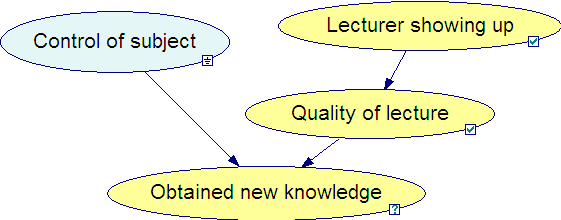
\includegraphics[scale=0.45]{obtain_knowledge.png}
\end{figure}
\\
Note that whether we obtain new knowledge or not is highly dependent on the
decision node controlling if we actually go to the lecture or not. By not going
the probability of obtaining new knowledge is zero.  Hence we need a dependency
from ‘Go to lecture’ to ‘Obtained new knowledge’, not shown in the figure
above.

The probability of the lecturer not showing up is 4\%, a value found by
analyzing lectures so far in various courses and our experience with soon three
years at the Norwegian University of Technology and Science.  Given that the
lecturer shows up, the probability of a good lecture is 20\%, a average lecture
is 60\% and a bad lecture is 20\%.  These numbers are based on the same grounds
as above. If the lecturer does not show up - the probability of a bad lecture
is of course 100\%.

Perhaps the most interesting node properties in this sub-system, which we are
focusing on here, is the probabilities defining when we obtain new knowledge.
We both agreed that the highest potential for learning is when we have average
control of the subject and the quality of the lecture is high.

\begin{table}[h]
  \centering
  \begin{tabular}{|c||c|c|c|} \hline
    Go to lecture & \multicolumn{3}{|c|}{Yes} \\ \hline
    Control of subject & \multicolumn{3}{|c|}{Some} \\ \hline
    Quality of lecture & Low & Medium & High \\ \hline \hline
    None & 0.3 & 0.1 & 0.05 \\ \hline
    Some & 0.5 & 0.45 & 0.3 \\ \hline
    Lots & 0.2 & 0.45 & 0.65 \\ \hline
  \end{tabular}
\end{table}

Let us draw our focus now on another important section of our model, namely our physical shape,
which of course plays a large role when deciding whether to stay home or not. 
\\
\begin{figure}[h]
  \centering
  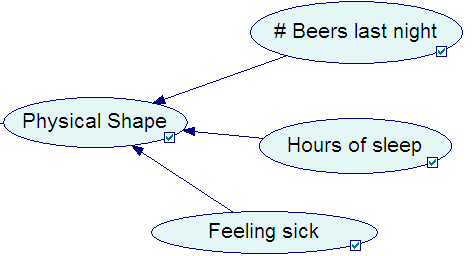
\includegraphics[scale=0.45]{physical_shape.png}
\end{figure}
\\
As one can see there are three factors which affect our physical shape, namely
the amount of beers consumed the night before, the amount of sleep and our
general feeling (are we feeling sick?). Notably if you are feeling sick our
physical form is generally characterized as bad, the only exception being when
you’ve slept a reasonably amount of time.  An interesting discussion took place
regarding probabilities of sleep and amount of beer. In general the numbers are
highly independent and hence important to change if you want the system to
depict your own life situation. An example is shown; Martin and Herman has the
following probabilities regarding alcohol:

\begin{table}[h]
  \centering
  \begin{tabular}{|c|c|c|} \hline
    & Martin & Herman \\ \hline
    Number of beers & \multicolumn{2}{|c|}{Probability} \\ \hline \hline
    0 & 0.35 & 0.55 \\ \hline
    1-2 & 0.2 & 0.1 \\ \hline
    1-2 & 0.2 & 0.1 \\ \hline
    3-4 & 0.1 & 0.05 \\ \hline
    5-6 & 0.15 & 0.2 \\ \hline
    7+ & 0.2 & 0.1 \\ \hline
  \end{tabular}
\end{table}

\newpage
Which yields the following results (when no evidence is set):

\begin{table}[h]
  \centering
  \begin{tabular}{|c|c|c|} \hline
    & Martin & Herman \\ \hline
    Go to lecture? & \multicolumn{2}{|c|}{Less than a month to exam} \\ \hline \hline
    Yes & 22.99 & 23.99 \\ \hline
    No & 7.17 & 6.04 \\ \hline
  \end{tabular}
\end{table}

Considering the fact that ten other probabilities are affecting our utility
function, a difference of 1 between Herman and Martin due to a small change in
alcohol habits is a strong verification on how important the independent
variables are in our model (and for life in general). They should both
generally go to the lectures, but since Herman is drinking less -- he is more
likely to show up. We could experiment with different values for both ‘feeling
sick’ and ‘amount of sleep’, but we’ll keep the discussion short and let that
be an exercise for the reader.

Finally, the weather is an important factor for both us and our friends. Hence
those nodes are affecting our utility function as well as the uncertain
variable ‘friends showing up’. Notice too that a friend may be feeling sick
(just as we may be), but this variable can not be the same as the one connected
to ‘Physical Shape’, even though they contain the same probabilities. If it
were connected to both nodes it would translate to ‘the probability for our
friend being sick at the same time as we are feeling sick’ -- which, of course,
is not what we want.

For both the precipitation and degrees we used a 50\% chance for
precipitation/no-precipitation and below 0 degrees/above 0 degrees,
respectively. This way the model works in a general season and these two nodes
need to be tuned with respect to city and season.  For example you would have a
high probability for precipitation in the autumn (especially in Trondheim)
compared to the summer.

A brief discussion of the utility function is appropriate. As mentioned in the
introduction our decision problem is based on a lot of properties, all except
one is discussed above. The remaining factor is the actual decision of going to
the lecture or not.  Why? The answer is simply shown with an example. Assume
that we are feeling really bad, it is cold outside and raining.  Now the
utility function has to depict a higher value for staying home (in order to
feel better), rather than attending the lecture -- and hence the actual
attendance affect our result. 

An interesting property was found when entering probabilities for the different
definitions. By placing ‘Go to lecture’ on the top we observed that the utility
function, or rather the values, was inversed depending on weather we attended
the lecture or not.  That is given the same properties we obtained the inverse
utility value. This is illustrated well with a random example:

\begin{table}[h]
  \centering
  \begin{tabular}{|c|c|c|} \hline
    Go to lecture? & \emph{Yes} & \emph{No} \\ \hline
    Obtained new knowledge & No & No \\ \hline
    Physical shape & Bad & Bad \\ \hline
    Friend showing up & No & No \\ \hline
    Days left to exam & More than two months & More than two months \\ \hline
    Degrees centigrade & Below 0 & Below 0 \\ \hline
    Precipitation & No & No \\ \hline
    {\bf Value } & -55 & 55 \\ \hline
  \end{tabular}
\end{table}

Our finished model ended up looking like the figure below. Please consult the
GeNiE file for details regarding the model:
\\
\begin{figure}[h]
  \centering
  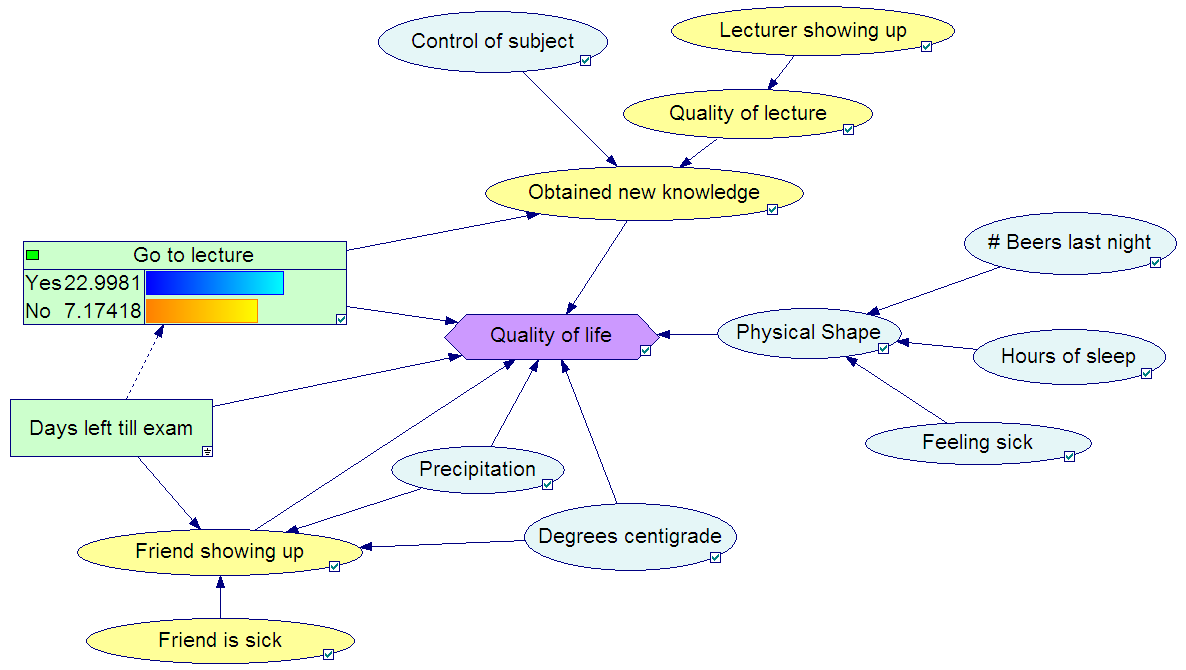
\includegraphics[scale=0.29]{model.png}
\end{figure}
\\
In this figure we've cleared all evidence and set the number of days till exam
to be 'Less than a month'.

\section*{Problems encountered}

We encountered numerous problems when doing this exercise, many of which might
be rooted in our relative inexperience in dealing with bayesian networks. At
first we gave every variable way too many possible states, e.g. degrees
centigrade had five different states.  This resulted in enormous amounts of
different states to consider in the utility-function, and we had to simplify to
just above and below zero degrees centigrade. This made it actually possible to
consider the different states in the utility function, but made our model much
simpler, perhaps even too simple to be a good tool in a real world situation.
We found that balancing these concerns was very complicated, especially since
adding just a single extra state to a variable directly considered in the
utility function increased the state-space enormously.

Even with the “simplified” state-space we ended up with, the amount of states
meant populating the utility function was a rather large data entry job. This
lead to us not being able to really ponder every possibility as much as we
would like, possibly skewing the results to some degree.

In general we found GeNIe to be somewhat frustrating to work with. For one, it
was Windows only -- forcing us to use IDI's terminal server which added some
headaches, and we would have much prefered to have implemented this ourselves
in a programming language or framework of our choosing.

\section*{Dicussion of results}

That we chose to be two students co-operating on this exercise posed a few
concerns. For example, the amount of sleep each of us needs to feel good the
next day is not nearly comparable, and one of us in general drinks more than
the other. As shown earlier, we tried with different values for the variables
where we behave differently, yielding at times significantly differing results.
In the end, we had to compromise and chose values that we felt represented the
pair of us in the most accurate manner.

Generally the model behaved as we wanted it to, even with the discrepancies
discussed. If we set evidence to seven or more beers, less than four hours
sleep etcetera, we end up with a recommendation of not going to the lecture. If
however we've slept well, hold back on drinking and the weather is fair, the
model recommends attending as expected. 

\end{document}
